\documentclass[11pt,a4paper]{article}

% =============================================================================
% PACKAGES
% =============================================================================
\usepackage[margin=1in]{geometry}
\usepackage[T1]{fontenc}
\usepackage{lmodern}
\usepackage{parskip}
\usepackage{enumitem}
\usepackage{xcolor}
\usepackage{amsmath, amssymb}
\usepackage[colorlinks=true,
            linkcolor=blue!60!black,
            urlcolor=blue!60!black,
            citecolor=blue!60!black]{hyperref}
\usepackage{listings}
\usepackage{tikz}
\usepackage[breakable,skins]{tcolorbox}
\usepackage{fancyhdr}
\usepackage{mdframed}
\usepackage{graphicx}
\usepackage{titlesec}
\usepackage{array}
\usepackage{longtable}
\usepackage{booktabs}

\usetikzlibrary{arrows.meta, positioning, shapes.geometric, fit, backgrounds, calc}
\pgfdeclarelayer{background}
\pgfsetlayers{background,main}

% =============================================================================
% LISTINGS (CODE) STYLING
% =============================================================================
\definecolor{codebg}{HTML}{F7F7F9}
\definecolor{codekw}{HTML}{1F4E79}
\definecolor{codestr}{HTML}{8E1B1B}
\definecolor{codecom}{HTML}{6A737D}

\lstdefinestyle{pycode}{
  language=Python,
  backgroundcolor=\color{codebg},
  basicstyle=\ttfamily\footnotesize,
  keywordstyle=\color{codekw}\bfseries,
  stringstyle=\color{codestr},
  commentstyle=\color{codecom}\itshape,
  showstringspaces=false,
  breaklines=true,
  frame=single,
  rulecolor=\color{black!20},
  numbers=left,
  numberstyle=\tiny\color{black!50},
  xleftmargin=2em,
  framexleftmargin=1.5em,
}

\lstset{style=pycode}

% Allow line breaks inside \texttt{} so long paths/function signatures don't
% overflow into the margin.
\sloppy
\emergencystretch=3em
\hyphenpenalty=2000
\exhyphenpenalty=2000
\hbadness=10000

% =============================================================================
% CALLOUT BOXES
% =============================================================================
\newtcolorbox{conceptbox}[1]{
  colback=yellow!8,
  colframe=yellow!50!orange,
  fonttitle=\bfseries,
  title={Concept: #1},
  breakable
}
\newtcolorbox{coderef}[1]{
  colback=blue!4,
  colframe=blue!40!black,
  fonttitle=\bfseries,
  title={In the code: #1},
  breakable
}
\newtcolorbox{defensebox}[1]{
  colback=green!4,
  colframe=green!40!black,
  fonttitle=\bfseries,
  title={Defense: #1},
  breakable
}
\newtcolorbox{pitfallbox}[1]{
  colback=red!4,
  colframe=red!50!black,
  fonttitle=\bfseries,
  title={Pitfall: #1},
  breakable
}
\newtcolorbox{intuitionbox}[1]{
  colback=purple!4,
  colframe=purple!45!black,
  fonttitle=\bfseries,
  title={Intuition: #1},
  breakable
}

% =============================================================================
% HEADERS / FOOTERS
% =============================================================================
\setlength{\headheight}{14pt}
\pagestyle{fancy}
\fancyhf{}
\fancyhead[L]{Navier--Stokes PINN --- Defender's Guide}
\fancyhead[R]{\thepage}
\fancyfoot[C]{Rishabh Kumar --- Personal Reference Document}
\renewcommand{\headrulewidth}{0.4pt}

\titlespacing*{\section}{0pt}{2.5ex plus 1ex minus .2ex}{1.5ex plus .2ex}
\titlespacing*{\subsection}{0pt}{2ex plus 1ex minus .2ex}{1ex plus .2ex}

% Convenience math macros for the recurring symbols.
\newcommand{\pd}[2]{\frac{\partial #1}{\partial #2}}
\newcommand{\pdd}[2]{\frac{\partial^2 #1}{\partial #2^2}}
\newcommand{\relL}{\text{rel-}L^2}

% =============================================================================
% TITLE
% =============================================================================
\title{\textbf{Hidden Fluid Mechanics}\\[0.5em]
       \large A Defender's Guide to the\\
       Inverse Navier--Stokes Physics-Informed Neural Network}
\author{Rishabh Kumar}
\date{Compiled \today}

\begin{document}
\maketitle

\begin{abstract}
\noindent This document is a complete, ground-up walkthrough of the Week~4
Navier--Stokes Physics-Informed Neural Network (PINN) project. It is written
for a reader who can read Python but has \emph{not} personally derived the
mathematics or internalised how the pieces fit together. The goal is twofold:
(1)~build a genuine understanding of every component from first principles ---
partial differential equations, automatic differentiation, the physics of
fluids, and the PINN idea itself --- and (2)~equip the reader to defend every
claim on the r\'esum\'e in a technical interview.

The document has five parts. \textbf{Part~I} builds the mathematical and
machine-learning foundations from near zero: what a derivative and a partial
differential equation are, what a neural network is, what gradient descent
does, and --- crucially --- what \emph{automatic differentiation} is and why
it is the engine that makes the whole project possible. \textbf{Part~II}
explains the physics: the Navier--Stokes equations term by term, what
incompressibility means, and the Taylor--Green vortex we use as ground truth.
\textbf{Part~III} explains the PINN idea and the two clever tricks that make
this project work: turning a PDE into a loss function, and the
\emph{stream-function} formulation that guarantees mass conservation exactly.
\textbf{Part~IV} is the codebase walkthrough --- a native pipeline diagram
plus a file-by-file, function-by-function tour that maps every line of code
back to the theory. \textbf{Part~V} is the interview-defence kit: every
r\'esum\'e claim defended with evidence, a bank of likely questions with model
answers, a glossary, and a one-page cheat sheet for last-minute revision.

Five kinds of callout boxes recur throughout: purple \textit{Intuition} boxes
give the plain-English picture before the maths, yellow \textit{Concept} boxes
introduce a piece of jargon for the first time, blue \textit{In the code} boxes
point you to exact files and line numbers, green \textit{Defense} boxes give
you the one-line answer to a likely interview question, and red
\textit{Pitfall} boxes flag things the system does \emph{not} do (and how to
talk about them honestly).
\end{abstract}

\vspace{1em}
\hrule
\vspace{1em}

\noindent\textbf{How to use this document:}
\begin{itemize}[leftmargin=2em]
  \item \textbf{First read} (one or two sittings, cover to cover): Part~I
        builds the vocabulary and maths; Part~II applies it to the physics;
        Part~III explains the PINN method; Part~IV walks the actual code;
        Part~V crystallises everything into interview-ready answers. Do not
        skip Part~I even if some of it feels basic --- the interview questions
        that trip people up are the foundational ones (``what \emph{is} a
        PINN, really?'').
  \item \textbf{Revision before an interview} (20--40 minutes): read the cheat
        sheet in Section~\ref{sec:cheatsheet}, then the Q\&A bank in
        Section~\ref{sec:qa}, then skim the green \textit{Defense} boxes.
  \item \textbf{Targeted lookup:} use the table of contents; every section is
        hyperlinked.
\end{itemize}

\newpage
\tableofcontents
\newpage

% =============================================================================
% PART I --- FOUNDATIONS
% =============================================================================
\part{Foundations (from the ground up)}
\label{part:foundations}

\section{What we built, in one paragraph}
\label{sec:what-we-built}

We built a neural network that solves the equations of fluid motion. More
precisely: given only a handful of \emph{noisy velocity measurements} scattered
around a 2D fluid flow, the system reconstructs (a)~the complete velocity field
everywhere in space and time, (b)~the \emph{pressure} field, which was never
measured at all, and (c)~an unknown physical constant --- the fluid's viscosity
--- which was also never given. It does this not by fitting a curve to data in
the usual machine-learning way, but by forcing the network to obey the actual
laws of physics (the Navier--Stokes equations) at thousands of points in the
domain. This is the ``hidden fluid mechanics'' idea: hidden quantities
(pressure, viscosity) fall out for free because the network is constrained by
the same equations the real fluid obeys.

\vspace{0.5em}
\noindent\textbf{In one sentence:} \emph{Sparse noisy velocity in;
full velocity field, unmeasured pressure, and an unknown viscosity out ---
by making a neural network obey the Navier--Stokes equations.}

\begin{intuitionbox}{The one analogy to remember}
Imagine you can only feel the surface ripples of a stream in a few random
spots. From just those touches, you deduce the entire current everywhere,
\emph{plus} the water pressure you never felt, \emph{plus} how thick/sticky the
water is. You can only pull that off because you \emph{know the laws of fluid
motion} and insist your reconstructed flow obeys them everywhere. The neural
network is your reconstruction; the Navier--Stokes equations are the laws you
insist on. Everything else in this document is detail on how that insistence is
implemented.
\end{intuitionbox}

\section{The problem this solves, and why it is impressive}
\label{sec:why-impressive}

There are two classes of problem in physics simulation:

\begin{description}[leftmargin=2em, style=nextline]
  \item[The forward problem] You know the equations and all the conditions
    (initial state, boundary behaviour, material constants). You want to
    compute how the system evolves. This is what a normal fluid simulator
    does.
  \item[The inverse problem] You have some \emph{measurements} of the outcome
    but you are \emph{missing} something --- maybe a material constant, maybe a
    field you couldn't measure. You want to work backwards to recover the
    missing pieces. This is much harder and much more valuable, because in the
    real world you almost never know everything up front.
\end{description}

Our project does \emph{both}, in two phases. Phase~1 (forward) is a warm-up
that proves our physics engine is correct. Phase~2 (inverse) is the headline:
it recovers hidden fields and an unknown constant from sparse, noisy data. The
inverse problem is what makes this r\'esum\'e-worthy --- it is the same class of
problem as medical imaging (reconstruct tissue from limited scans) or
geophysics (find oil from seismic echoes).

\begin{defensebox}{``What makes this hard / interesting?''}
``It's an inverse problem on the hardest classic PDE. From only sparse, noisy
velocity samples I reconstruct the full velocity field, recover the pressure
field which was never measured, and identify an unknown viscosity --- all
simultaneously. Pressure and viscosity aren't fit to data; they emerge because
I constrain the network to satisfy the Navier--Stokes equations everywhere.
That's the `hidden fluid mechanics' result --- the same idea used in medical
imaging and geophysics, where you recover what you can't directly measure by
enforcing known physics.''
\end{defensebox}

\section{Mathematical foundations you need}
\label{sec:math-foundations}

The next subsections build every mathematical idea the project rests on. Read
them in order the first time; treat them as a glossary later.

\subsection{Functions of several variables}
\label{sec:multivar}

Our unknowns are \emph{fields}: quantities that vary over space and time. The
horizontal velocity $u$ is not a single number; it is a function
$u(x, y, t)$ --- give it a location $(x,y)$ and a time $t$, and it returns the
horizontal speed of the fluid there and then. Likewise $v(x,y,t)$ (vertical
velocity) and $p(x,y,t)$ (pressure). The entire project is about finding these
three functions.

A neural network, it turns out, is also just a function: you feed it numbers,
it returns numbers. That coincidence is the whole trick --- we will use a
network \emph{as} the function $u,v,p$.

\subsection{Derivatives and partial derivatives}
\label{sec:derivatives}

\begin{intuitionbox}{What a derivative is}
A derivative is a \emph{rate of change} --- how fast one quantity changes as you
nudge another. If $f(x)$ is your height as you walk east, $\frac{df}{dx}$ is the
steepness of the ground under your feet. Positive means uphill, negative means
downhill, zero means flat.
\end{intuitionbox}

When a function has several inputs, a \emph{partial derivative} measures the
rate of change with respect to \emph{one} input while holding the others fixed.
We write $\pd{u}{x}$ (often abbreviated $u_x$) for ``how fast $u$ changes as we
move in the $x$-direction, at a fixed time and fixed $y$.'' The symbols you will
see constantly in this project:

\begin{itemize}[leftmargin=2em]
  \item $u_t = \pd{u}{t}$ --- how the velocity changes over \emph{time}
        (acceleration-like).
  \item $u_x = \pd{u}{x}$, $u_y = \pd{u}{y}$ --- how velocity changes across
        \emph{space}.
  \item $u_{xx} = \pdd{u}{x}$ --- a \emph{second} derivative: the rate of change
        of the rate of change. It measures \emph{curvature}. Second derivatives
        appear in the viscous (friction) term of Navier--Stokes.
\end{itemize}

\begin{conceptbox}{Why second derivatives = diffusion}
The combination $u_{xx} + u_{yy}$ (called the \emph{Laplacian}) measures how
much a point's value differs from the average of its neighbours. If a spot is a
``peak'' relative to its surroundings, the Laplacian is negative and diffusion
pulls it down; if it's a ``dip'', the Laplacian is positive and diffusion fills
it in. This is exactly how viscosity smooths out a fluid --- fast regions drag
slow neighbours along and vice versa. So when you see $\nu(u_{xx}+u_{yy})$ in
the equations, read it as ``viscous smoothing, with strength $\nu$.''
\end{conceptbox}

\subsection{What a partial differential equation (PDE) is}
\label{sec:pde}

An \emph{ordinary} differential equation (ODE) relates a function of \emph{one}
variable to its derivatives --- e.g.\ Newton's law of cooling,
$\frac{dT}{dt} = -k(T - T_{\text{env}})$, says ``the rate a cup cools is
proportional to how much hotter it is than the room.'' (This was the earlier,
simpler project in this repo.)

A \emph{partial} differential equation (PDE) relates a function of \emph{several}
variables to its partial derivatives. The Navier--Stokes equations are PDEs:
they relate the velocity and pressure fields to their space and time
derivatives. Solving a PDE means finding the actual function(s) $u,v,p$ that
make the equation true at \emph{every} point in the domain.

\begin{intuitionbox}{A PDE is a local rulebook}
A PDE doesn't tell you the answer directly. It gives you a \emph{local rule}
that the answer must satisfy at every point --- like ``at every spot, the way
velocity changes in time must equal this specific combination of how it changes
in space.'' Find a function that obeys the rule everywhere, and you've solved
the PDE. A PINN finds such a function by \emph{penalising} rule violations until
there are (almost) none left.
\end{intuitionbox}

\subsection{Neural networks as universal function approximators}
\label{sec:nn}

A neural network is a stack of simple operations: multiply the inputs by a
matrix of \emph{weights}, add a \emph{bias} vector, then apply a non-linear
\emph{activation function} (we use $\tanh$), and repeat for several
\emph{layers}. The final layer outputs the answer.

\begin{equation}
\mathbf{h}_0 = \text{input};\qquad
\mathbf{h}_{k+1} = \tanh(W_k \mathbf{h}_k + \mathbf{b}_k);\qquad
\text{output} = W_L \mathbf{h}_L + \mathbf{b}_L .
\end{equation}

The \emph{universal approximation theorem} says that a network with enough
hidden units can approximate essentially any continuous function to any desired
accuracy, \emph{provided} you can find the right weights. ``Finding the right
weights'' is called \emph{training}, and it is done by gradient descent.

\begin{conceptbox}{Why $\tanh$ and not ReLU}
Most modern networks use ReLU ($\max(0,x)$), but PINNs use smooth activations
like $\tanh$. The reason is central to this project: we need to take
\emph{second derivatives} of the network's output (for the $u_{xx}$ terms).
ReLU has a kink at $0$ and its second derivative is zero almost everywhere ---
useless for encoding curvature. $\tanh$ is infinitely differentiable, so its
higher derivatives are smooth and informative. \textbf{This is a genuine, often-asked interview point.}
\end{conceptbox}

\subsection{Gradient descent and the loss function}
\label{sec:gradient-descent}

Training means adjusting the weights to make the network's output ``good.''
``Good'' is quantified by a \emph{loss function} $\mathcal{L}$ --- a single
number that is large when the network is wrong and small when it is right.
Training minimises $\mathcal{L}$.

The tool is \emph{gradient descent}. The \emph{gradient}
$\nabla_\theta \mathcal{L}$ is the vector of partial derivatives of the loss
with respect to every weight $\theta$; it points in the direction of steepest
\emph{increase} of the loss. So we step the weights a little in the
\emph{opposite} direction:

\begin{equation}
\theta \leftarrow \theta - \eta \, \nabla_\theta \mathcal{L},
\end{equation}

where $\eta$ is the \emph{learning rate} (step size). Repeat thousands of times
and the loss (usually) drifts down to a minimum.

\begin{intuitionbox}{Descending a foggy hill}
You're on a hill in thick fog and want the valley. You can't see far, but you
can feel the slope under your feet (that's the gradient). Take a small step
downhill, re-check the slope, step again. That's gradient descent. The learning
rate is your stride length: too big and you overshoot the valley; too small and
you take forever.
\end{intuitionbox}

\subsection{The keystone: automatic differentiation}
\label{sec:autodiff}

This is the single most important concept in the entire project. Read it twice.

Everything above needs derivatives in two different places, and \emph{both} are
supplied by the same mechanism:

\begin{enumerate}[leftmargin=2em]
  \item Gradient descent needs $\nabla_\theta \mathcal{L}$ --- the derivative of
        the loss with respect to the weights.
  \item Our loss itself is built from the \emph{physics}, which needs
        derivatives of the network's \emph{output} with respect to its
        \emph{inputs} --- $u_t, u_x, u_{xx}$, etc.
\end{enumerate}

Both are computed by \emph{automatic differentiation} (autodiff), the technology
inside PyTorch. Autodiff is not numerical approximation (it does not use
$\frac{f(x+h)-f(x)}{h}$), and it is not symbolic algebra (it does not manipulate
formulas). Instead, as your code runs, PyTorch records every elementary
operation into a \emph{computational graph}, then applies the chain rule
backwards through that graph to get \emph{exact} derivatives (to machine
precision).

\begin{conceptbox}{The computational graph}
When you write \texttt{y = a * b + c} in PyTorch with ``\texttt{requires\_grad}''
tensors, PyTorch silently builds a little graph: two input nodes $a,b$ feed a
multiply node, whose result and $c$ feed an add node, producing $y$. Because it
knows the derivative rule for each elementary node (multiply, add, $\tanh$,
$\cos$, \ldots), it can walk the graph backward and compose those rules via the
chain rule to compute $\pd{y}{a}$, $\pd{y}{b}$, etc.\ exactly. This backward
walk is what \texttt{loss.backward()} does, and what
\texttt{torch.autograd.grad(...)} does on demand.
\end{conceptbox}

\begin{intuitionbox}{Why this is the magic of PINNs}
In a normal fluid simulator you approximate $u_{xx}$ with a grid: you sample $u$
at neighbouring grid points and take differences. That introduces grid error and
ties you to a mesh. In a PINN, $u$ \emph{is} a formula (the network), so autodiff
gives you $u_{xx}$ \emph{exactly}, at \emph{any} point $(x,y,t)$ you like, with
no mesh at all. That is why a PINN is called \emph{mesh-free}, and why it can
evaluate the physics at arbitrary scattered points. Autodiff is the enabling
technology --- without it, PINNs are impossible.
\end{intuitionbox}

\begin{coderef}{The autodiff call that powers everything --- \texttt{src/pde.py:8--16}}
The whole project's derivative machinery is one seven-line function:
\begin{lstlisting}[style=pycode]
def grad(outputs, inputs):
    return torch.autograd.grad(
        outputs, inputs,
        grad_outputs=torch.ones_like(outputs),
        create_graph=True,     # keep the graph so we can differentiate AGAIN
        retain_graph=True,
    )[0]
\end{lstlisting}
The critical flag is \texttt{create\_graph=True}. It tells PyTorch to build a
\emph{new} graph \emph{for the derivative itself}, so that we can differentiate
the derivative --- exactly what we need for the second-order terms $u_{xx}$
(\texttt{grad(grad(u, x), x)}). Every physics term in the project is ultimately
a stack of these \texttt{grad} calls. \textbf{If an interviewer asks ``how do
you compute the PDE derivatives,'' the answer is this function.}
\end{coderef}

% =============================================================================
% PART II --- THE PHYSICS
% =============================================================================
\part{The Physics}
\label{part:physics}

\section{The Navier--Stokes equations, term by term}
\label{sec:ns-equations}

The Navier--Stokes equations describe how a fluid moves. They are ``the hardest
classic PDE'' --- so hard that whether smooth solutions always exist in 3D is a
famous unsolved Millennium Prize problem. We work with the 2D, incompressible,
non-dimensional form. There are three equations: two momentum equations (one per
direction) and one continuity equation.

\subsection{The momentum equations (Newton's second law for fluids)}

\begin{align}
\underbrace{u_t}_{\text{unsteady}}
+ \underbrace{u\,u_x + v\,u_y}_{\text{convection}}
&= \underbrace{-\,p_x}_{\text{pressure}}
+ \underbrace{\nu\,(u_{xx} + u_{yy})}_{\text{viscous diffusion}}
\label{eq:mom-x}\\[4pt]
v_t + u\,v_x + v\,v_y
&= -\,p_y + \nu\,(v_{xx} + v_{yy})
\label{eq:mom-y}
\end{align}

Each momentum equation is $F = ma$ written for a tiny parcel of fluid. Reading
Equation~\eqref{eq:mom-x} left to right:

\begin{description}[leftmargin=2em, style=nextline]
  \item[$u_t$ --- unsteady term] How the horizontal velocity at a fixed point
    changes over time. This is the ``acceleration'' part.
  \item[$u\,u_x + v\,u_y$ --- convection (advection)] The fluid carries its own
    momentum around. A parcel speeds up or slows down simply by moving into a
    region where the velocity is different. \emph{This is the nonlinear term}
    (velocity multiplies its own derivative), and nonlinearity is precisely what
    makes fluids turbulent and the equations hard.
  \item[$-p_x$ --- pressure gradient] Fluid accelerates from high pressure to
    low pressure. The force is the \emph{negative gradient} of pressure. This is
    the only place pressure enters --- which is why, later, we can recover
    pressure from velocity: it's pinned by this relationship.
  \item[$\nu(u_{xx}+u_{yy})$ --- viscous diffusion] Internal friction smooths the
    velocity field, with strength set by the viscosity $\nu$. Recall from
    Section~\ref{sec:derivatives} that the Laplacian $u_{xx}+u_{yy}$ is a
    smoothing operator.
\end{description}

\begin{conceptbox}{What $\nu$ (viscosity) physically is}
$\nu$ (Greek ``nu'') is the \emph{kinematic viscosity} --- how thick or sticky
the fluid is. Honey has high $\nu$; water has low $\nu$; air lower still. In our
problem $\nu$ is the \emph{unknown constant} we recover in the inverse problem.
A larger $\nu$ means the flow's energy dissipates faster. This link between
$\nu$ and the \emph{rate of decay} is exactly what makes $\nu$ recoverable from
velocity data alone (Section~\ref{sec:why-nu-identifiable}).
\end{conceptbox}

\subsection{The continuity equation (conservation of mass)}

\begin{equation}
u_x + v_y = 0
\label{eq:continuity}
\end{equation}

This says the fluid is \emph{incompressible}: you cannot squeeze mass into a
point or create it from nothing. The quantity $u_x + v_y$ is the
\emph{divergence} of the velocity --- the net rate at which fluid flows
\emph{out} of an infinitesimal box. Setting it to zero means whatever flows in
must flow out; mass is conserved.

\begin{intuitionbox}{Divergence, concretely}
Picture a tiny box in the fluid. $u_x$ is how much faster fluid exits the right
face than it enters the left; $v_y$ is the same top-to-bottom. If their sum were
positive, mass would be piling up outside the box (impossible for an
incompressible fluid); if negative, mass would be vanishing. Zero divergence =
mass is conserved everywhere. Enforcing this is a genuine headache in fluid
solvers --- and Section~\ref{sec:stream-function} shows the elegant trick we use
to satisfy it \emph{exactly} and for free.
\end{intuitionbox}

\section{The Taylor--Green vortex: our ground truth}
\label{sec:tgv}

To test any solver you need a problem whose exact answer you already know. The
\emph{Taylor--Green vortex} (TGV) is one of the very few flows for which the
Navier--Stokes equations have a closed-form analytical solution. On the square
domain $[0, 2\pi]^2$ with periodic boundaries:

\begin{align}
u(x,y,t) &= -\cos(x)\sin(y)\,e^{-2\nu t}, \label{eq:tgv-u}\\
v(x,y,t) &= \phantom{-}\sin(x)\cos(y)\,e^{-2\nu t}, \label{eq:tgv-v}\\
p(x,y,t) &= -\tfrac{1}{4}\big(\cos(2x)+\cos(2y)\big)\,e^{-4\nu t}. \label{eq:tgv-p}
\end{align}

This is a grid of counter-rotating vortices (whirlpools). The spatial pattern
($\cos\sin$, $\sin\cos$) sets where the vortices are; the exponential factor
$e^{-2\nu t}$ makes them \emph{decay over time} as viscosity dissipates their
energy. Note the pressure decays twice as fast ($e^{-4\nu t}$).

\begin{conceptbox}{Why the decay rate is the key to the whole inverse problem}
Look at where $\nu$ appears: \emph{only} inside the decay exponent $e^{-2\nu t}$.
This means the \emph{speed at which the vortices fade} directly encodes $\nu$. If
you watch the flow at several instants and see how fast it decays, you can back
out $\nu$. This single observation is why sampling across \emph{multiple time
slices} is mandatory for the inverse problem --- one snapshot can't reveal a
decay rate. Remember this; it is the crux of Section~\ref{sec:why-nu-identifiable}.
\end{conceptbox}

\begin{coderef}{TGV in code --- \texttt{src/data.py:21--38}}
The analytical formulas are implemented exactly as above:
\begin{lstlisting}[style=pycode]
def tgv_velocity(x, y, t, nu):
    decay = torch.exp(-2.0 * nu * t)
    u = -torch.cos(x) * torch.sin(y) * decay
    v =  torch.sin(x) * torch.cos(y) * decay
    return u, v

def tgv_pressure(x, y, t, nu):
    return -0.25 * (torch.cos(2.0*x) + torch.cos(2.0*y)) * torch.exp(-4.0*nu*t)
\end{lstlisting}
These functions serve two roles: they generate the ``measurements'' we feed the
inverse problem (velocity only, plus noise), and they provide the ground truth we
compare against when reporting accuracy.
\end{coderef}

% =============================================================================
% PART III --- THE PINN IDEA
% =============================================================================
\part{The PINN Idea and Its Two Key Tricks}
\label{part:pinn}

\section{Turning a PDE into a loss function}
\label{sec:pde-to-loss}

Here is the conceptual leap that defines a Physics-Informed Neural Network. We
have a network that outputs candidate fields. How do we make it output the
\emph{right} fields --- the ones that solve Navier--Stokes?

\textbf{Idea:} rearrange each PDE so one side is zero, then treat the other side
as an error to be minimised. Take the $x$-momentum equation and move everything
to one side:

\begin{equation}
f_u \;:=\; u_t + u\,u_x + v\,u_y + p_x - \nu(u_{xx}+u_{yy}).
\label{eq:residual-u}
\end{equation}

If the network's outputs perfectly solve the physics, then $f_u = 0$ everywhere.
If they don't, $f_u \neq 0$, and its magnitude measures \emph{how badly} the
physics is violated at that point. We call $f_u$ the \emph{residual}. Define
$f_v$ analogously for the $y$-momentum equation.

Now build a loss: sample many scattered points (called \emph{collocation}
points), compute the residuals there via autodiff, and average their squares:

\begin{equation}
\mathcal{L}_{\text{PDE}} = \frac{1}{N}\sum_{i=1}^{N}
\Big( f_u(x_i,y_i,t_i)^2 + f_v(x_i,y_i,t_i)^2 \Big).
\label{eq:pde-loss}
\end{equation}

Minimising $\mathcal{L}_{\text{PDE}}$ with gradient descent \emph{pushes the
residuals toward zero}, i.e.\ forces the network to satisfy the equations. That
is the entire PINN principle.

\begin{intuitionbox}{The physics is the teacher}
In ordinary supervised learning, labelled data is the teacher: ``here is the
right answer at these points.'' In a PINN, the \emph{equations} are the teacher:
``I won't tell you the answer, but I'll penalise you wherever you break the laws
of physics.'' The remarkable consequence is that a PINN can find the solution in
regions where you have \emph{no data at all}, because the physics constrains it
there too.
\end{intuitionbox}

\begin{coderef}{The residual --- \texttt{src/pde.py:31--61}}
\texttt{navier\_stokes\_residual} is Equation~\eqref{eq:residual-u} in code. It
calls the network, extracts velocities, then stacks \texttt{grad} calls to build
every derivative and assemble $f_u, f_v$:
\begin{lstlisting}[style=pycode]
u_t = grad(u, t); u_x = grad(u, x); u_y = grad(u, y)
u_xx = grad(u_x, x); u_yy = grad(u_y, y)      # second derivatives
# ... same for v, and p_x, p_y ...
f_u = u_t + u*u_x + v*u_y + p_x - nu*(u_xx + u_yy)
f_v = v_t + u*v_x + v*v_y + p_y - nu*(v_xx + v_yy)
\end{lstlisting}
Note \texttt{nu} can be a fixed number (forward problem) \emph{or} a learnable
tensor (inverse problem) --- the same residual code serves both, which is why
the codebase is compact.
\end{coderef}

\section{Key trick \#1: the stream-function formulation}
\label{sec:stream-function}

Recall the continuity equation $u_x + v_y = 0$ (mass conservation). We could add
it as a third residual term and hope the optimiser drives it to zero. But there
is a far better way that makes it \emph{exactly} zero, for free, forever.

\textbf{The trick:} instead of having the network output $u$ and $v$ directly,
have it output a single scalar field $\psi$ (the \emph{stream function}) and
define velocity as its derivatives:

\begin{equation}
u = \psi_y, \qquad v = -\psi_x.
\label{eq:stream-def}
\end{equation}

Now substitute into the continuity equation and watch what happens:

\begin{equation}
u_x + v_y = \pd{}{x}(\psi_y) + \pd{}{y}(-\psi_x)
          = \psi_{yx} - \psi_{xy} = 0.
\label{eq:continuity-exact}
\end{equation}

The last step uses the fact that mixed partial derivatives are equal
($\psi_{yx} = \psi_{xy}$, Clairaut's theorem) for any smooth $\psi$. So
continuity holds \emph{identically} --- not approximately, not ``after
training,'' but as an algebraic identity, no matter what the network does. We
have eliminated an entire equation and guaranteed physical correctness by
construction.

\begin{center}
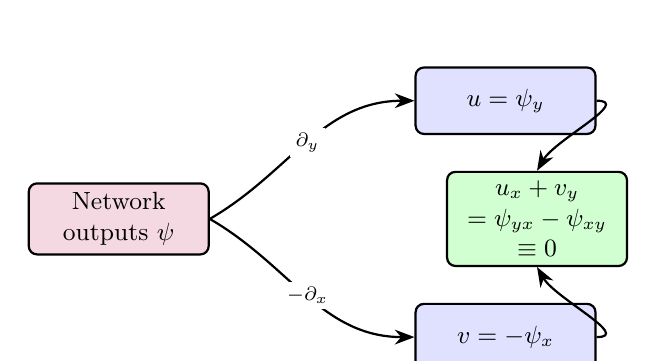
\begin{tikzpicture}[
  every node/.style={font=\small, align=center},
  box/.style={draw, rounded corners=3pt, minimum height=2.4em,
              minimum width=6.5em, thick},
  arr/.style={-{Stealth[length=2.5mm]}, thick},
  op/.style={font=\scriptsize\itshape, midway, fill=white, inner sep=2pt}
]
  \node[box, fill=purple!15] (net) {Network\\outputs $\psi$};
  \node[box, fill=blue!12, above right=0.6 and 2.6 of net] (u) {$u = \psi_y$};
  \node[box, fill=blue!12, below right=0.6 and 2.6 of net] (v) {$v = -\psi_x$};
  \node[box, fill=green!18, right=3.0 of net] (cont)
       {$u_x + v_y$\\$= \psi_{yx}-\psi_{xy}$\\$\equiv 0$};

  \draw[arr] (net.east) to[out=30,in=180] node[op]{$\partial_y$} (u.west);
  \draw[arr] (net.east) to[out=-30,in=180] node[op]{$-\partial_x$} (v.west);
  \draw[arr] (u.east) to[out=0,in=60] (cont.north);
  \draw[arr] (v.east) to[out=0,in=-60] (cont.south);
\end{tikzpicture}
\end{center}

\begin{defensebox}{``Why a stream function instead of predicting $u,v$ directly?''}
``If I predict $u$ and $v$ directly, mass conservation $u_x+v_y=0$ is an extra
constraint I'd have to add as another loss term and hope the optimiser balances
it against the others. Instead I have the network output a stream function
$\psi$ and set $u=\psi_y,\, v=-\psi_x$. Then $u_x+v_y = \psi_{yx}-\psi_{xy}=0$
identically, because mixed partials commute. So incompressibility is satisfied
\emph{exactly by construction} --- one fewer loss term to balance and a big
stability win. In the code I verify the divergence is about $10^{-9}$, i.e.\
machine precision.''
\end{defensebox}

\begin{coderef}{Stream-function head --- \texttt{src/pde.py:19--28}}
\begin{lstlisting}[style=pycode]
def velocity_from_stream(psi, x, y):
    psi_x = grad(psi, x)
    psi_y = grad(psi, y)
    u = psi_y          # u =  d(psi)/dy
    v = -psi_x         # v = -d(psi)/dx
    return u, v
\end{lstlisting}
The network (\texttt{src/model.py}) outputs two numbers per point: $\psi$ and
$p$. Velocity is \emph{derived} from $\psi$ by this function, so it is never
predicted directly --- which is what makes continuity automatic.
\end{coderef}

\section{Key trick \#2: input normalisation against spectral bias}
\label{sec:normalization}

Neural networks have a known weakness called \emph{spectral bias}: they learn
smooth, low-frequency patterns easily but struggle with high-frequency detail.
Our domain is $[0, 2\pi]$, and the solution wiggles (it's made of $\cos$ and
$\sin$). To help the network, we \emph{normalise} the inputs from their raw
range $[0, 2\pi]$ to $[-1, 1]$ before they enter the network. This keeps the
network operating in the range where $\tanh$ and its gradients are well-behaved,
which noticeably improves convergence.

\begin{coderef}{Input normalisation --- \texttt{src/model.py:41--47}}
\begin{lstlisting}[style=pycode]
def _normalize(self, inp):
    return 2.0 * (inp - self.in_low) / (self.in_high - self.in_low) - 1.0
\end{lstlisting}
\texttt{in\_low} and \texttt{in\_high} are the domain bounds
$(0,0,0)$ and $(2\pi, 2\pi, T)$, registered as buffers so they move to the GPU
with the model. This maps each of $x,y,t$ linearly onto $[-1,1]$.
\end{coderef}

% =============================================================================
% PART IV --- THE CODEBASE
% =============================================================================
\part{The Codebase, End to End}
\label{part:codebase}

\section{The pipeline at a glance}
\label{sec:pipeline}

Before the file-by-file tour, here is the end-to-end data flow for the
\emph{inverse} problem (the headline). Every box maps to a module you'll meet
below; keep this diagram bookmarked.

\begin{figure}[h!]
\centering
\scalebox{0.86}{%
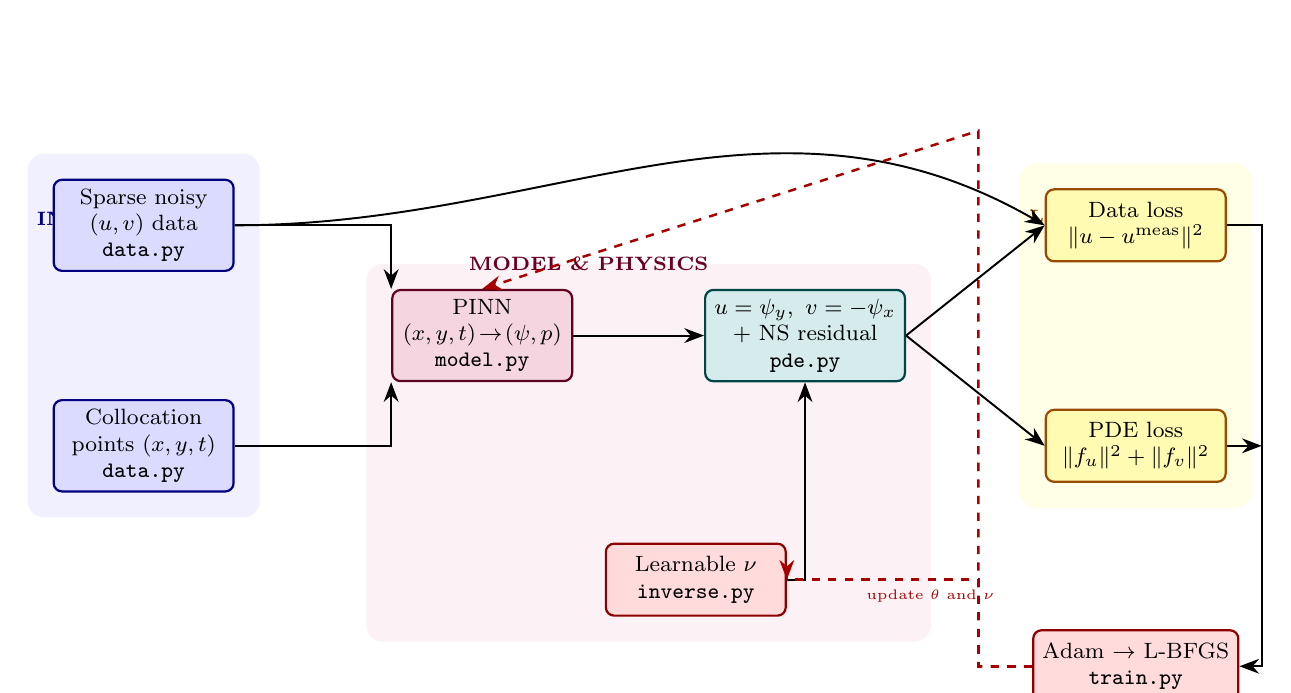
\begin{tikzpicture}[
  every node/.style={font=\footnotesize, align=center},
  data/.style={draw=blue!50!black, rounded corners=3pt, fill=blue!14,
               minimum height=2.6em, minimum width=6.5em, thick, line width=0.8pt},
  model/.style={draw=purple!50!black, rounded corners=3pt, fill=purple!16,
                minimum height=2.6em, minimum width=6.5em, thick, line width=0.8pt},
  phys/.style={draw=teal!55!black, rounded corners=3pt, fill=teal!16,
               minimum height=2.6em, minimum width=6.5em, thick, line width=0.8pt},
  loss/.style={draw=orange!60!black, rounded corners=3pt, fill=yellow!30,
               minimum height=2.6em, minimum width=6.5em, thick, line width=0.8pt},
  opt/.style={draw=red!55!black, rounded corners=3pt, fill=red!14,
              minimum height=2.6em, minimum width=6.5em, thick, line width=0.8pt},
  arr/.style={-{Stealth[length=2.5mm]}, thick, line width=0.7pt},
  dasharr/.style={-{Stealth[length=2.5mm]}, thick, dashed, red!65!black, line width=0.9pt},
  band/.style={rounded corners=6pt, inner sep=9pt},
  bandlbl/.style={font=\scriptsize\bfseries, anchor=west}
]

  % --- Inputs (left) ---
  \node[data] (meas) at (0, 1.4) {Sparse noisy\\$(u,v)$ data\\\texttt{data.py}};
  \node[data] (coll) at (0, -1.4) {Collocation\\points $(x,y,t)$\\\texttt{data.py}};

  \begin{pgfonlayer}{background}
    \node[band, fill=blue!6, fit=(meas)(coll),
          label={[bandlbl, blue!50!black]above left:INPUTS}] {};
  \end{pgfonlayer}

  % --- Network + stream head ---
  \node[model] (net)  at (4.3, 0) {PINN\\$(x,y,t)\!\to\!(\psi,p)$\\\texttt{model.py}};
  \node[phys]  (uv)   at (8.4, 0) {$u=\psi_y,\ v=-\psi_x$\\ + NS residual\\\texttt{pde.py}};
  \node[opt, right=0.4 of net, yshift=-3.1cm] (nu) {Learnable $\nu$\\\texttt{inverse.py}};

  \begin{pgfonlayer}{background}
    \node[band, fill=purple!5, fit=(net)(uv)(nu),
          label={[bandlbl, purple!55!black]above left:MODEL \& PHYSICS}] {};
  \end{pgfonlayer}

  % --- Loss ---
  \node[loss] (ldata) at (12.6, 1.4)  {Data loss\\$\|u-u^{\text{meas}}\|^2$};
  \node[loss] (lpde)  at (12.6, -1.4) {PDE loss\\$\|f_u\|^2+\|f_v\|^2$};

  \begin{pgfonlayer}{background}
    \node[band, fill=yellow!10, fit=(ldata)(lpde),
          label={[bandlbl, orange!60!black]above left:LOSS \texttt{(inverse.py)}}] {};
  \end{pgfonlayer}

  % --- Optimizer ---
  \node[opt] (opt) at (12.6, -4.2) {Adam $\to$ L-BFGS\\\texttt{train.py}};

  % --- Arrows ---
  \draw[arr] (meas.east) -- (net.west |- meas.east) -- (net.north west);
  \draw[arr] (coll.east) -- (net.west |- coll.east) -- (net.south west);
  \draw[arr] (net) -- (uv);
  \draw[arr] (nu.east) -| (uv.south);
  \draw[arr] (uv.east) -- (ldata.west);
  \draw[arr] (uv.east) -- (lpde.west);
  % measurements also compared in the data loss
  \draw[arr] (meas.east) to[out=0,in=150] (ldata.west);

  % losses -> optimizer
  \draw[arr] (ldata.east) -- (14.2,1.4) -- (14.2,-4.2) -- (opt.east);
  \draw[arr] (lpde.east)  -- (14.2,-1.4);

  % optimizer updates network + nu (gradient descent), dashed feedback
  \draw[dasharr] (opt.west) -- (10.6,-4.2) -- (10.6,-3.1) --
       node[below, font=\tiny, pos=0.25]{update $\theta$ and $\nu$} (nu.east |- 10.6,-3.1) -- (nu.east);
  \draw[dasharr] (opt.west) -- (10.6,-4.2) -- (10.6, 2.6) -- (net.north);

\end{tikzpicture}%
}
\caption{Inverse-problem data flow. Sparse noisy velocity measurements and
scattered collocation points (blue) feed the PINN, which outputs $(\psi,p)$;
velocity is derived from $\psi$ and the Navier--Stokes residual is formed using
the \emph{learnable} viscosity $\nu$ (purple/teal). Two loss terms (yellow) --- a
data misfit on the measurements and the PDE residual at collocation points ---
are summed and minimised by the two-stage Adam~$\to$~L-BFGS optimiser (red),
whose gradients update \emph{both} the network weights $\theta$ and $\nu$ (dashed
feedback). Pressure has no loss term of its own --- it is recovered purely
through the residual's pressure-gradient coupling. The forward problem
(Phase~1) is the same picture with $\nu$ fixed and the data loss replaced by
initial-condition + periodic-boundary losses.}
\label{fig:pinn-pipeline}
\end{figure}

\section{File-by-file tour}
\label{sec:file-tour}

The codebase lives under \texttt{Week4/src/} (the library) with two driver
scripts (\texttt{run\_forward.py}, \texttt{run\_inverse.py}) at
\texttt{Week4/}. Here is what each file does and why.

\begin{description}[leftmargin=1.5em, style=nextline]
  \item[\texttt{src/config.py} --- All the knobs in one place]
    A single \texttt{@dataclass Config} holding the physics (true $\nu=0.01$,
    domain $[0,2\pi]^2$, time $[0,2]$), sampling counts, network shape
    ($8\times 64$ by default), optimiser settings, loss weights, and the random
    seed. Centralising these means every experiment is reproducible and every
    number is traceable. \texttt{\_\_post\_init\_\_} packs the domain bounds
    into \texttt{domain\_lows}/\texttt{domain\_highs} tuples used by the model's
    normaliser.

  \item[\texttt{src/utils.py} --- Reproducibility and the accuracy metric]
    Three small functions: \texttt{set\_seed} (seeds Python, NumPy, Torch so runs
    are repeatable), \texttt{get\_device} (picks the GPU if available), and
    \texttt{relative\_l2} --- the error metric we report everywhere,
    $\|\text{pred}-\text{true}\|_2 / \|\text{true}\|_2$.

  \item[\texttt{src/data.py} --- Ground truth, samplers, and noisy measurements]
    Implements the TGV analytical fields (Section~\ref{sec:tgv}) and every
    sampler: \texttt{sample\_collocation} (interior points for the residual),
    \texttt{sample\_initial} (the $t=0$ slice for the forward IC),
    \texttt{sample\_boundary} (matched opposite-edge pairs for periodicity),
    \texttt{sample\_measurements} (the sparse, noisy velocity data for the
    inverse problem --- pressure never produced here), and
    \texttt{grid\_eval\_points} (a dense grid for evaluation and plotting).

  \item[\texttt{src/model.py} --- The neural network]
    The \texttt{PINN} class: a $\tanh$ MLP mapping $(x,y,t)\to(\psi,p)$, with
    Xavier weight initialisation, input normalisation to $[-1,1]$, and inputs
    taken as \emph{three separate column tensors} (so autograd can differentiate
    w.r.t.\ each coordinate independently). It outputs two numbers: $\psi$ (the
    stream function) and $p$ (pressure).

  \item[\texttt{src/pde.py} --- The physics engine]
    The heart of the project. \texttt{grad} (the autodiff helper of
    Section~\ref{sec:autodiff}), \texttt{velocity\_from\_stream} (the
    stream-function head of Section~\ref{sec:stream-function}),
    \texttt{navier\_stokes\_residual} (the momentum residuals of
    Section~\ref{sec:pde-to-loss}), and \texttt{predict\_uvp} (a convenience
    that returns $(u,v,p)$ at any points).

  \item[\texttt{src/inverse.py} --- Learnable viscosity and inverse loss]
    \texttt{LearnableNu} wraps $\nu$ as a trainable parameter kept positive via
    softplus (Section~\ref{sec:learnable-nu}); \texttt{inverse\_loss} is the
    data-misfit + PDE-residual loss with \emph{no} pressure, IC, or BC terms;
    \texttt{nu\_error} reports the relative error of the recovered $\nu$.

  \item[\texttt{src/train.py} --- The training loops]
    Both the forward (\texttt{train}) and inverse (\texttt{train\_inverse})
    two-stage Adam~$\to$~L-BFGS loops, the loss assemblers
    (\texttt{forward\_loss}), and the batch builders. Also logs the loss history
    and, for the inverse run, the $\nu$ trajectory.

  \item[\texttt{src/viz.py} --- All the plots]
    \texttt{plot\_field\_comparison} (exact vs PINN vs absolute-error triptych),
    \texttt{plot\_vorticity}, \texttt{plot\_loss\_curve}, and
    \texttt{plot\_param\_curve} (the $\nu$-convergence figure).

  \item[\texttt{run\_forward.py} / \texttt{run\_inverse.py} --- The drivers]
    Top-level scripts that wire everything together, run training, evaluate,
    save figures, and write \texttt{results/metrics.json}. These are what you
    actually execute to reproduce the results.
\end{description}

\begin{coderef}{Where to look first when changing X}
\begin{itemize}[leftmargin=2em]
  \item ``Change the viscosity, domain, or network size'' $\to$
        \texttt{src/config.py}.
  \item ``Change how the physics residual is built'' $\to$
        \texttt{src/pde.py}: \texttt{navier\_stokes\_residual}.
  \item ``Change the inverse loss or how $\nu$ is parameterised'' $\to$
        \texttt{src/inverse.py}.
  \item ``Change how many measurements / how much noise'' $\to$
        \texttt{run\_inverse.py} constants \texttt{N\_MEAS}, \texttt{NOISE}.
  \item ``Change the optimiser schedule'' $\to$ \texttt{src/train.py}.
\end{itemize}
\end{coderef}

\section{The model in detail}
\label{sec:model-detail}

\begin{coderef}{\texttt{src/model.py:44--51} --- the forward pass}
\begin{lstlisting}[style=pycode]
def forward(self, x, y, t):
    h = self._normalize(torch.cat([x, y, t], dim=1))  # -> [-1,1]
    for layer in self.linears[:-1]:
        h = self.activation(layer(h))                 # tanh hidden layers
    out = self.linears[-1](h)                          # linear output layer
    psi = out[:, 0:1]                                  # stream function
    p   = out[:, 1:2]                                  # pressure
    return psi, p
\end{lstlisting}
\end{coderef}

Three design choices worth being able to explain:

\begin{enumerate}[leftmargin=2em]
  \item \textbf{Separate $x,y,t$ inputs, concatenated inside.} The caller passes
        three column tensors, each with \texttt{requires\_grad=True}. This lets
        autodiff compute $\pd{\cdot}{x}$, $\pd{\cdot}{y}$, $\pd{\cdot}{t}$
        independently --- essential for building the residual.
  \item \textbf{Two outputs $(\psi, p)$, not three $(u,v,p)$.} Velocity is
        derived from $\psi$ (the stream-function trick), so the network only
        needs to output the scalar potential $\psi$ and the pressure.
  \item \textbf{Xavier initialisation, zero biases.} Standard, keeps early
        activations in a healthy range so gradients flow well from the start.
\end{enumerate}

\section{The inverse problem in detail}
\label{sec:inverse-detail}

\subsection{Making viscosity learnable}
\label{sec:learnable-nu}

Viscosity must stay positive (a negative viscosity is unphysical). But
optimisers work best on unconstrained variables. The solution: store an
unconstrained ``raw'' parameter and pass it through \emph{softplus}
($\text{softplus}(w) = \log(1+e^w)$, which is always positive) to get $\nu$.

\begin{coderef}{\texttt{src/inverse.py:14--33} --- \texttt{LearnableNu}}
\begin{lstlisting}[style=pycode]
class LearnableNu(nn.Module):
    def __init__(self, init=0.05):
        # invert softplus so nu STARTS exactly at `init`
        raw0 = math.log(math.expm1(init))
        self.raw = nn.Parameter(torch.tensor(float(raw0)))
    def forward(self):
        return F.softplus(self.raw)   # always > 0
\end{lstlisting}
We initialise at $\nu_0 = 0.05$ --- \emph{five times} the true value of $0.01$ ---
deliberately, so that recovering the truth is a genuine result, not a lucky
start. The \texttt{math.log(math.expm1(init))} line inverts softplus so that
$\nu$ begins exactly at \texttt{init}.
\end{coderef}

\subsection{The inverse loss (and what is deliberately absent)}
\label{sec:inverse-loss}

\begin{equation}
\mathcal{L}_{\text{inv}} =
\underbrace{\frac{1}{N_d}\sum \big(|u-u^{\text{meas}}|^2 + |v-v^{\text{meas}}|^2\big)}_{\text{data misfit (measured velocity only)}}
\;+\;
\underbrace{\frac{1}{N_c}\sum\big(f_u^2 + f_v^2\big)}_{\text{PDE residual}}.
\label{eq:inverse-loss}
\end{equation}

What is \emph{not} here is as important as what is:
\begin{itemize}[leftmargin=2em]
  \item \textbf{No pressure term.} We never tell the network what pressure is. It
        is forced into existence by the residual (see below).
  \item \textbf{No initial/boundary conditions.} Unlike the forward problem, the
        scattered data itself anchors the solution.
\end{itemize}

\begin{defensebox}{``How can you recover pressure if you never measured it?''}
``The momentum equations couple pressure to velocity: rearranged, they say the
pressure \emph{gradient} equals a specific combination of the velocity
derivatives, $p_x = \nu(u_{xx}+u_{yy}) - (u_t + uu_x + vu_y)$, and similarly for
$p_y$. Once the network has fit the measured velocity and the residual is driven
to zero, those equations pin down $p_x$ and $p_y$ everywhere --- which
determines pressure up to a constant. So pressure is recovered purely from
physics, with zero pressure data. That's the `hidden' in hidden fluid
mechanics.''
\end{defensebox}

\subsection{Why viscosity is identifiable}
\label{sec:why-nu-identifiable}

\begin{defensebox}{``Why can you recover $\nu$ from velocity alone?''}
``Because $\nu$ controls the \emph{decay rate}. In the Taylor--Green solution the
velocity amplitude is $e^{-2\nu t}$, so how fast the flow slows down directly
encodes $\nu$. That's why I sample measurements across \emph{multiple time
slices} $t\in[0,2]$ --- a single snapshot can't reveal a rate of decay, but
several can. During training, the only value of $\nu$ that makes the residual
consistent with the observed decay is the true one, so the optimiser is driven
to it. I start it 5$\times$ off (0.05 vs 0.01) and it recovers to within 3.9\%.''
\end{defensebox}

\subsection{The pressure gauge subtlety}
\label{sec:pressure-gauge}

In incompressible flow only the pressure \emph{gradient} $\nabla p$ appears in
the equations --- never $p$ itself. This means pressure is only defined up to an
arbitrary additive constant (you can add $100$ to the pressure everywhere and
the physics is unchanged). So when we report pressure error, we first subtract
the spatial mean from both the predicted and the true field; comparing absolute
pressure would be meaningless.

\begin{coderef}{Mean-subtraction --- \texttt{run\_inverse.py} (evaluate)}
\begin{lstlisting}[style=pycode]
p_p_c = p_p - p_p.mean()   # predicted, mean-subtracted
p_t_c = p_t - p_t.mean()   # true, mean-subtracted
# ... then relative_l2(p_p_c, p_t_c)
\end{lstlisting}
\textbf{This is a favourite ``gotcha'' interview question} --- knowing to
mean-subtract shows you understand the physics, not just the code.
\end{coderef}

\section{Training internals: Adam then L-BFGS}
\label{sec:training-internals}

We train in \emph{two stages}, and being able to explain why is a strong
interview point.

\begin{description}[leftmargin=2em, style=nextline]
  \item[Stage 1 --- Adam] A first-order, stochastic-friendly optimiser using
    only gradients. It is robust and good at escaping bad regions from a random
    start, but it converges slowly near the end and plateaus. We run it for a few
    thousand iterations with a \emph{plateau scheduler} that cuts the learning
    rate when progress stalls.
  \item[Stage 2 --- L-BFGS] A \emph{quasi-Newton} optimiser that approximates the
    curvature (second-order information) of the loss surface. Near a good
    solution it converges very fast and very precisely --- it ``snaps'' onto the
    minimum. It is expensive per step and needs a full-batch \emph{closure}, so
    it's used only for the final polish.
\end{description}

\begin{intuitionbox}{Why two stages}
Adam is like hiking roughly downhill in the fog --- reliable but it slows to a
crawl near the valley floor. L-BFGS is like switching to a precise instrument
once you're close, that reads the local curvature and steps straight to the
bottom. Adam gets you to the right neighbourhood cheaply; L-BFGS nails the exact
minimum. Using Adam alone leaves accuracy on the table; using L-BFGS alone from
a random start is unstable. The combination is a standard, cheap accuracy win.
\end{intuitionbox}

\begin{conceptbox}{What a ``closure'' is}
L-BFGS may evaluate the loss several times per step (it does a line search). So
PyTorch's L-BFGS asks you for a \emph{closure} --- a function it can call to
recompute the loss and gradients on demand. In \texttt{src/train.py} the nested
\texttt{closure()} function does exactly this: zero the gradients, recompute the
loss, call \texttt{backward()}, and return the loss.
\end{conceptbox}

For the inverse problem, the crucial detail is that \emph{both} the network
weights and $\nu$ are handed to the optimiser together:

\begin{coderef}{\texttt{src/train.py:146} --- joint optimisation}
\begin{lstlisting}[style=pycode]
params = list(model.parameters()) + list(nu_module.parameters())
optimizer = torch.optim.Adam(params, lr=cfg.adam_lr)
\end{lstlisting}
So gradient descent updates $\theta$ and $\nu$ simultaneously; the same loss that
shapes the field also drags $\nu$ toward its true value. The $\nu$-convergence
figure shows the two-phase signature clearly: a slow Adam drift, then a sharp
L-BFGS snap onto $0.01$ at the stage boundary.
\end{coderef}

% =============================================================================
% PART V --- INTERVIEW DEFENCE KIT
% =============================================================================
\part{Interview Defence Kit}
\label{part:defence}

\section{Every r\'esum\'e claim, defended}
\label{sec:claims-defended}

Your three r\'esum\'e bullets and the exact evidence behind each. All numbers
come from \texttt{Week4/results/metrics.json}.

\begin{longtable}{@{}p{0.42\textwidth} p{0.52\textwidth}@{}}
\toprule
\textbf{Claim} & \textbf{Evidence \& how to defend it} \\
\midrule
\endhead
Reconstructed full 2D Navier--Stokes velocity \& hidden pressure field from
sparse, noisy data to 1.6\% L2 &
From 4000 scattered velocity samples with 3\% noise (pressure hidden), the
recovered fields hit rel-$L^2$ of 0.42\% ($u$), 0.42\% ($v$), and 1.61\% ($p$,
mean-subtracted). Pressure was never in the loss --- it comes from the momentum
coupling (Section~\ref{sec:inverse-loss}). \\[4pt]
Recovered unknown viscosity to 3.9\% of ground truth from 3\%-noisy velocity
alone &
$\nu$ initialised at 0.05 (5$\times$ off), recovered to 0.0104 vs true 0.01 ---
a 3.86\% error. Identifiable because $\nu$ sets the decay rate $e^{-2\nu t}$ and
we sample across time (Section~\ref{sec:why-nu-identifiable}). \\[4pt]
Enforced exact mass conservation via a stream-function PINN, cutting field error
to 0.4\% L2 (Adam/L-BFGS) &
Stream-function head makes $u_x+v_y\equiv 0$ by construction (verified
$\sim 10^{-9}$); two-stage Adam~$\to$~L-BFGS drives velocity error to 0.42\%
(Sections~\ref{sec:stream-function}, \ref{sec:training-internals}). \\
\bottomrule
\end{longtable}

\begin{pitfallbox}{One phrase to NOT claim}
An early template mentioned \emph{``residual-based adaptive sampling.''} We did
\textbf{not} implement that (collocation points are sampled uniformly, once). It
is correctly \emph{absent} from your final r\'esum\'e bullets --- do not add it
back. If asked ``could you improve this?'', adaptive sampling (resampling
collocation points where the residual is largest) is a great, honest answer for
\emph{future} work.
\end{pitfallbox}

\section{Anticipated questions \& model answers}
\label{sec:qa}

\begin{description}[leftmargin=1.5em, style=nextline]
  \item[Q: What is a PINN in one sentence?]
    A neural network that represents the solution of a differential equation and
    is trained by penalising violations of that equation (computed via
    automatic differentiation) rather than, or in addition to, fitting labelled
    data.

  \item[Q: Where does the ``physics'' actually enter the training?]
    Through the loss. I plug the network's autodiff derivatives into the
    Navier--Stokes equations to form a residual, and minimising the squared
    residual forces the network to obey the physics at thousands of collocation
    points.

  \item[Q: Why is automatic differentiation essential here?]
    The PDE needs exact spatial/temporal derivatives of the solution
    ($u_t, u_x, u_{xx}, \ldots$). Because the network is a differentiable
    formula, autodiff gives those derivatives exactly and mesh-free, at any
    point. \texttt{create\_graph=True} lets me differentiate twice for the
    second-order viscous terms.

  \item[Q: Why $\tanh$ activation?]
    I need smooth second derivatives for the $u_{xx}$ terms. ReLU's second
    derivative is zero almost everywhere, so it can't represent curvature;
    $\tanh$ is infinitely differentiable.

  \item[Q: How do you guarantee mass conservation?]
    By construction, not by penalty. The network outputs a stream function
    $\psi$; velocity is $u=\psi_y,\, v=-\psi_x$, so $u_x+v_y=\psi_{yx}-\psi_{xy}
    \equiv 0$. I verified the divergence is $\sim 10^{-9}$.

  \item[Q: How can pressure be recovered without measuring it?]
    The momentum equations fix the pressure gradient in terms of velocity
    derivatives. Once velocity fits the data and the residual is minimised,
    pressure is determined up to a constant --- so I mean-subtract before scoring
    it.

  \item[Q: Why is $\nu$ recoverable, and why multiple time slices?]
    $\nu$ appears only in the decay rate $e^{-2\nu t}$. A single snapshot can't
    show a decay rate; sampling across time can, so $\nu$ becomes identifiable.

  \item[Q: Why Adam then L-BFGS?]
    Adam is robust from a random start but plateaus; L-BFGS uses curvature to
    converge precisely near the minimum. Adam gets close cheaply, L-BFGS nails
    the accuracy. It's also where $\nu$ snaps onto its true value.

  \item[Q: What are the limitations?]
    It's validated on the Taylor--Green vortex (a smooth analytical flow), not a
    turbulent or real-world dataset; collocation sampling is uniform, not
    adaptive; and PINNs in general can be slow to train and sensitive to loss
    weighting. These are honest, and each has a known remedy (harder datasets,
    adaptive sampling, loss balancing).

  \item[Q: How did you know your engine was correct before the inverse run?]
    Phase~1: I first solved the \emph{forward} Taylor--Green problem from physics
    alone (IC + periodic BC + PDE residual) and checked the result against the
    known analytical solution --- sub-1\% velocity error. That de-risked the
    residual code before the harder inverse problem.

  \item[Q: Isn't this just curve-fitting?]
    No --- there is no pressure data and no interior velocity labels in the
    inverse problem. The interior field, the pressure, and $\nu$ are all
    determined by enforcing the PDE, not by fitting targets. That's the
    difference between a PINN and ordinary regression.
\end{description}

\section{Glossary}
\label{sec:glossary}

\begin{description}[leftmargin=2em, style=nextline]
  \item[PINN] Physics-Informed Neural Network: a network trained to satisfy a
    differential equation via a residual loss.
  \item[PDE] Partial Differential Equation: relates a multivariable function to
    its partial derivatives.
  \item[Residual] The PDE rearranged to equal zero; its magnitude measures
    physics violation.
  \item[Collocation points] Scattered interior points where the PDE residual is
    enforced.
  \item[Autodiff (autograd)] Exact derivative computation by recording and
    reverse-traversing a computational graph.
  \item[Stream function $\psi$] A scalar whose derivatives give a
    divergence-free velocity field ($u=\psi_y,\, v=-\psi_x$).
  \item[Continuity / incompressibility] $u_x+v_y=0$; mass conservation.
  \item[Viscosity $\nu$] How ``sticky'' the fluid is; sets the viscous
    (diffusion) strength and the decay rate.
  \item[Vorticity $\omega$] $v_x-u_y$; local spinning of the fluid, a derived
    diagnostic.
  \item[Relative $L^2$ error] $\|\text{pred}-\text{true}\|_2/\|\text{true}\|_2$;
    our accuracy metric.
  \item[Taylor--Green vortex] An exact analytical solution of 2D Navier--Stokes
    used as ground truth.
  \item[Adam / L-BFGS] First-order / quasi-Newton optimisers; used in sequence.
  \item[Softplus] $\log(1+e^w)$; smooth positive function used to keep $\nu>0$.
  \item[Forward vs inverse problem] Forward: known everything, compute
    evolution. Inverse: recover missing fields/constants from partial data.
\end{description}

\section{One-page cheat sheet (last-minute revision)}
\label{sec:cheatsheet}

\begin{mdframed}[linewidth=0.8pt, roundcorner=4pt, backgroundcolor=black!2]
\small
\textbf{Elevator pitch.} ``I built an inverse Physics-Informed Neural Network for
2D incompressible Navier--Stokes. From sparse, noisy velocity samples only, it
reconstructs the full velocity field, the pressure field it never measured, and
an unknown viscosity --- because I constrain the network to obey the
Navier--Stokes equations everywhere.''

\medskip
\textbf{The five things to know cold:}
\begin{enumerate}[leftmargin=1.6em, noitemsep]
  \item \textbf{PINN idea:} rearrange the PDE to $f=0$, form residual via
    autodiff, minimise $f^2$ at collocation points $\Rightarrow$ physics as loss.
  \item \textbf{Autodiff:} exact, mesh-free derivatives of the network;
    \texttt{create\_graph=True} enables 2nd-order terms $u_{xx}$. This is the
    enabling tech.
  \item \textbf{Stream-function trick:} output $\psi$, set $u=\psi_y,v=-\psi_x$
    $\Rightarrow$ $u_x+v_y\equiv0$ exactly (mixed partials commute). Verified
    $\sim 10^{-9}$.
  \item \textbf{Inverse magic:} pressure from momentum coupling (no pressure
    data); $\nu$ from decay rate $e^{-2\nu t}$ (needs multiple time slices);
    mean-subtract $p$ (gauge freedom).
  \item \textbf{Training:} Adam (robust, coarse) $\to$ L-BFGS (curvature,
    precise). $\nu$ snaps to truth in the L-BFGS phase.
\end{enumerate}

\medskip
\textbf{Headline numbers.} $\nu$: 0.05 $\to$ 0.0104 (true 0.01, \textbf{3.9\%}
err). rel-$L^2$: \textbf{0.42\%} $u$, \textbf{0.42\%} $v$, \textbf{1.61\%} $p$
(mean-sub). Forward (Phase~1): 0.74\%/0.90\%/3.58\%. Setup: 4000 samples, 3\%
noise, $8\times64$ $\tanh$ MLP, domain $[0,2\pi]^2\times[0,2]$.

\medskip
\textbf{Why $\tanh$?} Need smooth 2nd derivatives. \textbf{Why 2 stages?} Adam
coarse + L-BFGS precise. \textbf{Why stream fn?} Free exact mass conservation.
\textbf{Why sample over time?} To make $\nu$ identifiable. \textbf{Not
implemented:} adaptive sampling (good ``future work'' answer).
\end{mdframed}

\vfill
\begin{center}\rule{0.4\textwidth}{0.4pt}\end{center}
\begin{center}\small\itshape
End of guide. To request changes, refer to a section by its number or label;
the table of contents on page~2 is the index and can absorb new sections.
\end{center}

\end{document}
